\documentclass[a4paper, 12pt]{article}
\usepackage[margin=24mm]{geometry}
\usepackage{float}
\usepackage{titling}
\usepackage{graphicx}
\usepackage{caption}
\usepackage{subcaption}
\usepackage{hyperref}
\usepackage[toc,page]{appendix}
\usepackage{multirow}
%
%\geometry{bindingoffset=35mm}

\begin{document}

\begin{titlepage}
\begin{center}{\LARGE
Electronics and Computer Science\\
Faculty of Physical and Applied Sciences\\
University of Southampton\\
\hfill \break
\hfill \break
\hfill \break\\
Merlin Webster\\
\today\\
\hfill \break
Skydiving Formation Recognition\\
\begin{figure}[H]
	\centering
	\includegraphics[width=.7\linewidth]{fs_silhouette.png}
\end{figure}
Project supervisor: Dr Jonathon S Hare\\
Second examiner: Prof Lie-Liang Yang\\
\hfill \break
\hfill \break
A project progress report submitted for the award of\\
MEng Electronic Engineering\\}
\end{center}
\end{titlepage}
%
\section{Introduction}
%
\section{Background}
Contrary to popular belief, skydiving is a competitive and technical sport, requiring careful control of body position in order to not only remain stable, but also to move around the sky in freefall in a controlled manner.\\
A popular discipline in the sport is formation skydiving (FS). This involves multiple skydivers forming set formations in freefall, in order to score as many points as possible. A point is awarded for each successful formation in a sequence \textbf{\emph{(see figure \ref{fig:fs_dive_pool})}}. In 4 person FS (4-way FS) each skydiver has a specific slot in the formation. This is the position that they will always take in order to make each formation. This is done in such a way to minimise the amount of movement required for each skydiver when transitioning between formations. The four slots in 4-way FS are Point, Tail, Outside Center (OC) and Inside Center (IC). 
%
In order for the team to create formations in the sky, it is important that they practice the skydive multiple times on the ground. This is known as "dirt diving" and is often done using partially triangular wheeled platforms that each skydiver lays on, known as "creepers"  \textbf{\emph{(see figures \ref{fig:creepers} and \ref{fig:creepers_use})}}.
\begin{figure}[H]
	\centering
	\begin{subfigure}{.5\textwidth}
		\centering
		\includegraphics[width=0.9\linewidth]{creepers.jpg}
		\caption{FS practice platforms "creepers"}
		\label{fig:creepers}
	\end{subfigure}%
	\begin{subfigure}{.5\textwidth}
		\centering
		\includegraphics[width=0.9\linewidth]{creepers_use.jpg}
		\caption{"Creepers" in use while "dirt diving" a "Donut" formation}
		\label{fig:creepers_use}
	\end{subfigure}
	\caption{Images reproduced from \url{www.skydivespaceland.com/blog/images/creepers2.jpg} and \url{www.skydiveaz.com/images/old-images/creepers.jpg}}
\end{figure}
%
	\subsection{Project Brief}
The original focus of the project was to analyse video of dirt diving and identify which formations have been performed. The focus has been modified, and is now to analyse footage of formation skydiving in a vertical wind tunnel, indoor skydiving. This change is due to the fact that the body position of a skydiver in the wind tunnel is exactly the same as that of a skydiver in freefall. The wind is turned up to freefall speeds, simulating the environment of a regular skydive, but in a much more controlled environment. Another benefit of analysing footage taken in a wind tunnel is that the camera is mounted above the formation, and remains static \textbf{\emph{(see figure \ref{fig:sample_tunnel})}}. The set of formations I will be analysing are the BPA rookie class of formations known as 'randoms'. The software must be able to recognise all 16 of the randoms \textbf{\emph{(see figure \ref{fig:fs_dive_pool})}}.
%
\begin{figure}[H]
	\centering
	\includegraphics[width=\linewidth]{FS_All.png}
	\caption{All 16 BPA rookie class FS 'randoms' formations, with their names. The colours for each slot are: Point red, OC green, IC blue, Tail yellow.\\
	Reproduced from \url{http://www.teamsatori.co.uk/New\%204W\%20Random\%20Dive\%20pool.pdf}}
	\label{fig:fs_dive_pool}
\end{figure}
%
\begin{figure}[H]
	\centering
	\begin{subfigure}{.5\textwidth}
		\centering
		\includegraphics[width=0.9\linewidth]{Tunnel_Star.png}
	\end{subfigure}%
	\begin{subfigure}{.5\textwidth}
		\centering
		\includegraphics[width=0.9\linewidth]{Tunnel_Sidebody.png}
	\end{subfigure}\\
	\begin{subfigure}{.5\textwidth}
		\centering
		\includegraphics[width=0.9\linewidth]{Tunnel_Phalanx.png}
	\end{subfigure}%
	\begin{subfigure}{.5\textwidth}
		\centering
		\includegraphics[width=0.9\linewidth]{Tunnel_Donut.png}
	\end{subfigure}%
	\caption{Sample FS formations performed in a wind tunnel, with their names.\\
	Images reproduced from International Bodyflight Association, \url{www.youtube.com/watch?v=Y2B4S3lGf54&list=LLsEkKn0qzIHSGefmSGT_4og}. }
	\label{fig:sample_tunnel}
\end{figure}
%
\section{Literature Report}
%
List sources...
How does generalised procrasts analysis work?\\
How do active shape and point distribution models work?\\
What am I using for skeletonisation?
\section{Proposed Final Design}
%
The proposed final design will take the form of a command line tool. It will take a video of formation skydiving to be analysed. It will output the same video file, but with an overlay showing which formations have been formed. It will also highlight the skeletons of the skydivers in different colours in order to show which slot in the formation they are flying. The skeletons will take the same colours as in \textbf{\emph{\ref{fig:fs_dive_pool}}}.
\section{Completed Work}
	\subsection{Data Collection}
	Software has been written that handles collection of data for the initial point 			matrix to be used to create the point distribution model. In order to speed up data collection, the program displays an image of a skydiver and asks the user to left click on different parts of the skydivers body. The user can undo the last point by right clicking. Once all the points for the image are recorded, they are written to an output file and form the next row of the initial point matrix. Another image is then shown and the process repeats. This is a console based application and takes the file path of an image list as its only input \textbf{\emph{(see figure \ref{fig:data_collection})}}. This image list is stored in an XML file, as OpenCV natively supports input and output to XML files. For each image, the program adds another row to the initial point matrix. This contains the coordinates of each point x1, y1, x2, y2, ... ,x11 ,y11 and stores the data for each new image in another row. Currently only 10 images have been used to create the initial point matrix, but this number will be increased before it is used to create the point distribution model.
%
\begin{figure}[H]
	\centering
	\includegraphics[width=\linewidth]{data_collection.png}
	\caption{Data labelling program. Screenshot taken once all the required points of the image had been clicked on.}
	\label{fig:data_collection}
\end{figure}
%
\begin{figure}[H]
	\centering
	\includegraphics[width=\linewidth]{initial_matrix.png}
	\caption{Matrix created when the program is supplied with a sample image list with 10 images in it.}
	\label{fig:initial_matrix}
\end{figure}
%
	\subsection{Skeletonisation}
	Software has been written that creates a minimal, connected, 1 pixel thick skeleton from a binary mask. The function uses a medial axis transformation based method \cite{skeletonisation}  to create the skeleton and the Ramer--–Douglas–--Peucker\cite{Ramer}\cite{Douglas_Peucker} (RDP) algorithm to minimise it.
%
\subsubsection{Skeletonisation Algorithm}
        \begin{enumerate}
   		\item Find all boundary pixels (edge of the binary mask) using a binary laplacian mask\cite{binary_laplacian}. For each boundary pixel do the following:
        \item{Test pixels neighbours
        %
\begin{table}[H]
\centering
\begin{tabular}{llll}
\cline{1-3}
\multicolumn{1}{|l|}{p8} & \multicolumn{1}{l|}{p1} & \multicolumn{1}{l|}{p2} & y \\ \cline{1-3}
\multicolumn{1}{|l|}{p7} & \multicolumn{1}{l|}{p0} & \multicolumn{1}{l|}{p3} &  \\ \cline{1-3}
\multicolumn{1}{|l|}{p6} & \multicolumn{1}{l|}{p5} & \multicolumn{1}{l|}{p4} & $\downarrow$ \\ \cline{1-3}
x &  & $\rightarrow$ & 
\end{tabular}
\end{table}}
%
        \item Count Np0, number of non-zero neighbours of p0.
        \item Count Tp0, number of 0-1 transitions in sequence p1, p2, ..., p8.
        \item Check the initial conditions; mark for deletion any point that satisfies them all.\\
        Initial conditions:
        \begin{itemize}
         \item $cA:     2 <= Np0 <= 6$
         \item $cB:     Tp1 = 1$
         \item $cC:     p1 . p3 . p5 = 0$
         \item $cD:     p3 . p5 . p7 = 0$
         \end{itemize} 
         
        \item Delete any points marked for deletion.
        \item For each remaining boundary pixel, recalculate Np0 and Tp0, then check secondary conditions; marking for deletion any point that satisfies them all:\\
Secondary conditions:
        \begin{itemize}
        \item $cA:     2 <= Np0 <= 6$
        \item $cB:     Tp1 = 1$
        \item $cC\_:    p1 . p3 . p7 = 0$
        \item $cD\_:    p1 . p5 . p7 = 0$
        \end{itemize}
        \item Delete any points marked for deletion.
        \end{enumerate}
%
Repeat process until no points are deleted.\\
For more a more in depth explanation of the algorithm, see \cite{skeletonisation}.
       
\subsubsection{Skeleton Simplification Algorithm}
	The RDP algorithm is designed to simplify a curve, while still maintaining its overall shape. A curve can be thought of as a collection of linked line segments, with each line segment stretching between two consecutive points on the curve. The basic principle of the algorithm is to reduce the number of line segments in a curve; creating a similar, but simplified curve. The algorithm is initially given an ordered array of all the points in the curve. The algorithm is also given the variable $\epsilon$; this defines the degree to which the curve should be simplified and represents a minimum distance between line segments on the curve. It marks the start and end points of the curve as the first line segment (L), and then finds the point furthest from this initial line segment. If the distance from this point to the line segment (d) is less than $\epsilon$ then it is marked for removal. If the point is further than $\epsilon$ then it is kept and the algorithm recursively called with this point as the new end point. In this way the algorithm is able to remove every point that is closer than $\epsilon$ to the line segment that joins its neighbours.
%
\begin{figure}[H]
	\centering
  	\includegraphics[width=\textwidth]{douglas_peucker.png}
  	\caption{Diagram showing the RDP algorithm working on a curve. 0 being the initial curve to be simplified, and 4 being the fourth result the algorithm. Red arrows show points marked for deletion, green arrows show points to be kept\\
  	Modified from \url{http://upload.wikimedia.org/wikipedia/commons/9/91/Douglas_Peucker.png}.}
  	\label{fig:douglas_peucker}
\end{figure}
%
\noindent The RDP algorithm is used to reduce the number of points in the skeleton, simplifying it.
However, it is only able to simplify curves with no bifurcations. This proves to be a problem when trying to simplify a skeleton produced by the skeltonisation algorithm, as it will always have bifurcations at the waist and neck. It may also also produce erroneous bifurcations at other points on the skeleton. These bifurcations can be seen in \textbf{\emph{figure \ref{fig:skel}}}.\\
The location of these bifurcations can be detected by applying a modified version of condition $cB$ from the skeletonisation algorithm. Tp0 is calculated in the same way, by looking at the number of 0-1 transitions in the sequence p1, p2, ... , p8.
%
\begin{table}[h]
\centering
\begin{tabular}{llll}
\cline{1-3}
\multicolumn{1}{|l|}{p8} & \multicolumn{1}{l|}{p1} & \multicolumn{1}{l|}{p2} & y \\ \cline{1-3}
\multicolumn{1}{|l|}{p7} & \multicolumn{1}{l|}{p0} & \multicolumn{1}{l|}{p3} &  \\ \cline{1-3}
\multicolumn{1}{|l|}{p6} & \multicolumn{1}{l|}{p5} & \multicolumn{1}{l|}{p4} & $\downarrow$ \\ \cline{1-3}
x &  & $\rightarrow$ & 
\end{tabular}
\end{table}
%
\\If $Tp0 > 2$ then a bifurcation is present at p0.
This is always true, as the skeletonisation algorithm ensures that the skeleton is a single pixel thick 8-connected component.\\
Once the location of every bifurcation is found, the skeleton can be split into separate curves, by removing the bifurcation point. The RDP algorithm is then run on each of these curves independently. The simplified curves can then be recombined to form a simplified skeleton. At this point it is also possible the remove the false skeleton sections created by the skeletonisation algorithm forming erroneous bifurcations. The simplest way to do this is to delete any simplified skeleton section that is shorter than a given length. This works as the false skeleton sections tend to be shorter than the correct ones. A more reliable method for detecting false skeleton sections could be used in the final design.
%
\begin{figure}[H]
	\centering
	\begin{subfigure}{.5\textwidth}
  		\centering
  		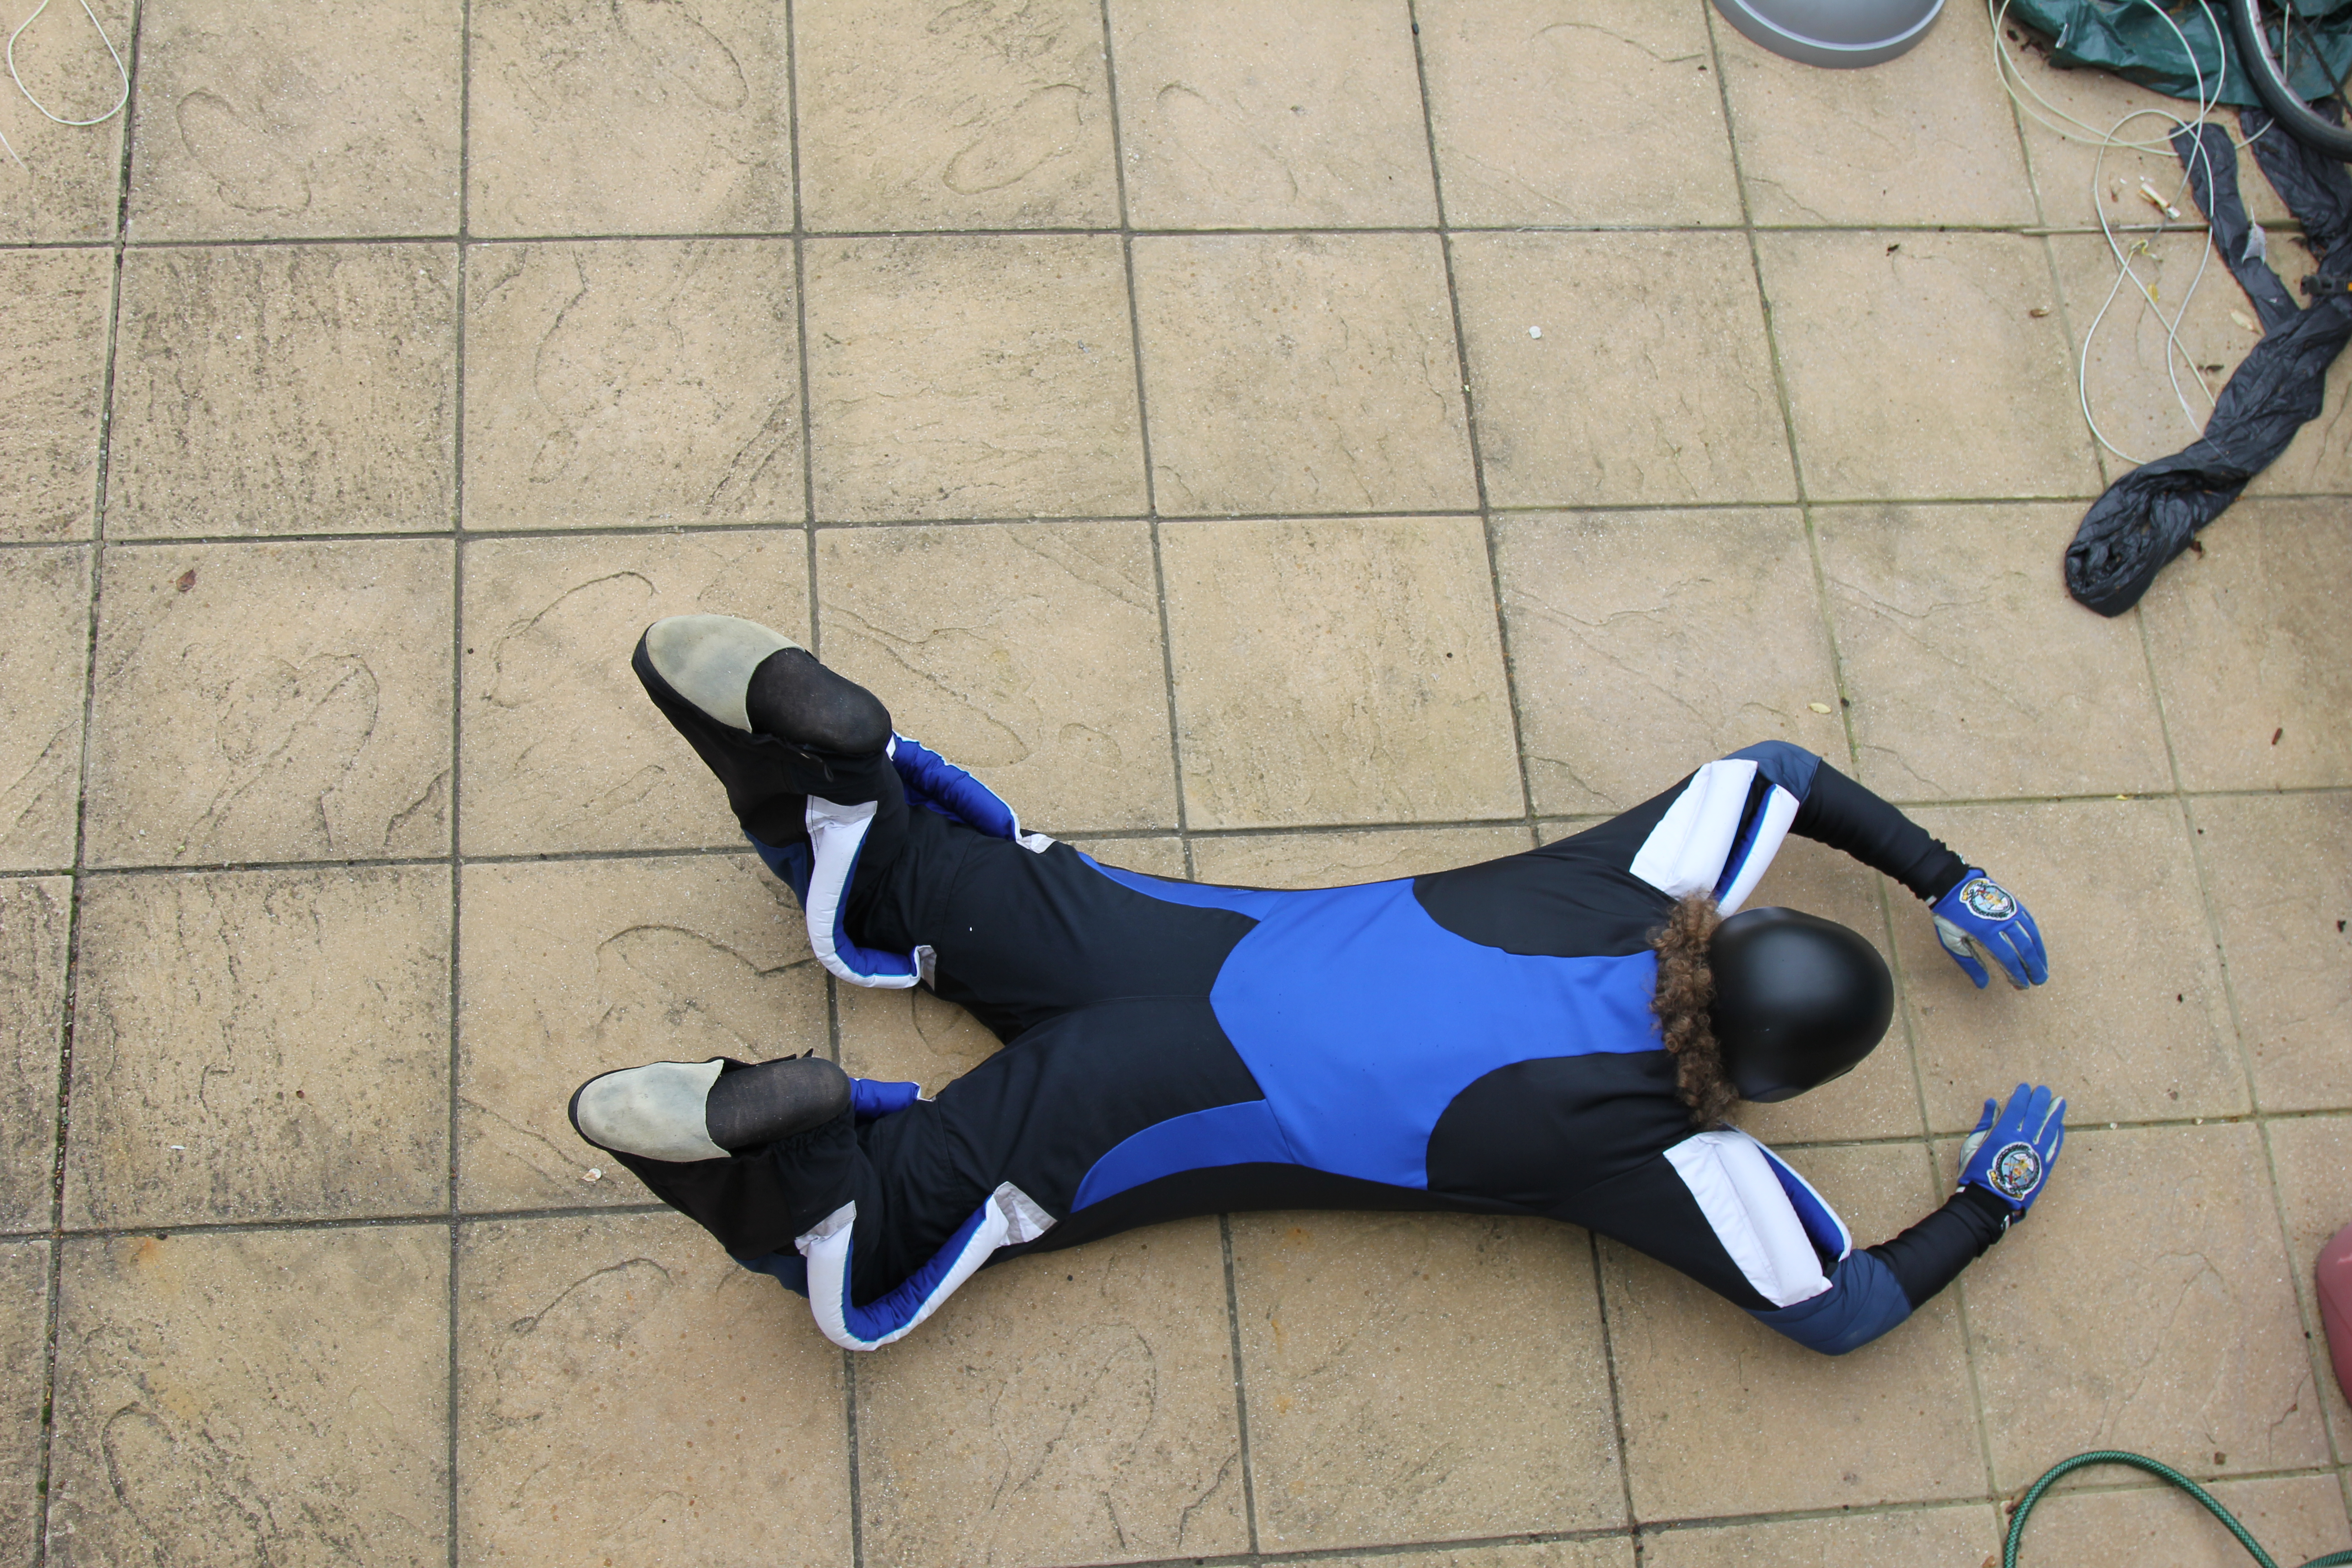
\includegraphics[width=.95\linewidth]{skel_src.jpg}
  		\caption{Skeletonisation source image}
  		\label{fig:skel_src}
	\end{subfigure}%
	%
	\begin{subfigure}{.5\textwidth}
  		\centering
  		\includegraphics[width=.95\linewidth]{skel_src_mask.jpg}
  		\caption{Binary mask of source image}
  		\label{fig:skel_src_mask}
	\end{subfigure}\\
	%
	\begin{subfigure}{.5\textwidth}
  		\centering
  		\includegraphics[width=.95\linewidth]{skel.jpg}
  		\caption{Result of skeletonisation function. Erroneous bifurcations are circled in red.}
  		\label{fig:skel}
	\end{subfigure}%
	%
	\begin{subfigure}{.5\textwidth}
  		\centering
  		\includegraphics[width=.95\linewidth]{skel_reduced.jpg}
  		\caption{Result of skeleton simplification algorithm}
  		\label{fig:skel_reduced}
	\end{subfigure}
\caption{}
\end{figure}
%
\section{Plan of Remaining Work}
%
\emph{\\\\\\An enhanced project description (development of the brief above).\\
A report on the background research and literature search.\\
The proposed final design of the system or experiment.\\
A justification for the approach.\\
An account of the work to date.\\
A plan of the remaining work.\\
An estimate of any support required to complete the project.\\
A Gantt chart showing the schedule of both completed and remaining work}.\\
%
%
%
%
%
%
%
\begin{thebibliography}{9}
\bibitem{skeletonisation}
    Rafael C. Gonzalez \& Richard E. Woods,
    "Skeletons",
    Digital Image Processing -- Second Edition --- International Edition (2001),
    pg650-653
%
\bibitem{binary_laplacian}
    Rafael C. Gonzalez \& Richard E. Woods,
    "The Laplacian",
    Digital Image Processing -- Second Edition --- International Edition (2001),
    pg581-585
%
\bibitem{Ramer}
    Urs Ramer,
    "An iterative procedure for the polygonal approximation of plane curves",
    Computer Graphics and Image Processing (1972),
    pg 244--–256
%
\bibitem{Douglas_Peucker}
	David Douglas \& Thomas Peucker,
	"Algorithms for the reduction of the number of points required to represent a 				digitized line or its caricature",
	The Canadian Cartographer (1973),
	pg112--–122
\end{thebibliography}
%
\begin{appendices}
%
\chapter{Gantt Charts}
\begin{figure}[H]
	\centering
	\includegraphics[width=\linewidth]{Gantt_initial_split.png}
	\caption{Initial Gantt Chart}
	\label{fig:gantt_initial}
\end{figure}
%
\end{appendices}
%
\end{document}